\documentclass[11pt]{article}
%Gummi|063|=)
\title{\textbf{Algorithms I -- supervision 7}}
\author{James Wood}
\usepackage{listings}
\usepackage{bold-extra}
\usepackage{xcolor}
\usepackage{amsmath}
\usepackage{enumitem}
\usepackage{tikz}
\usetikzlibrary{arrows}

\lstset{
  basicstyle=\small,
  basewidth=0.5em,
  frame=single,
  breaklines=true,
  %postbreak=\raisebox{0ex}[0ex][0ex]{
  %  \ensuremath{\color{red}\hookrightarrow\space}
  %}
  language=python,
  literate=
    {<=}{{\(\leq\)}}1
    {>=}{{\(\geq\)}}1
    {&&}{{\(\wedge\)}}1
    {||}{{\(\vee\)}}1
    {->}{{\(\rightarrow\)}}1
}

\tikzset{
  treenode/.style = {align=center, inner sep=0pt, text centered,
    font=\sffamily},
  bnode/.style = {treenode, circle, white, draw=black,
    fill=black, text width=1.5em},
  rnode/.style = {treenode, circle, red, draw=red,
    text width=1.5em, very thick},
  leaf/.style = {treenode, rectangle, draw=black,
    minimum width=0.5em, minimum height=0.5em}
}

\begin{document}
\renewcommand{\labelenumi}{(\alph{enumi})}
\renewcommand{\labelenumii}{(\roman{enumii})}

\maketitle

\section{Maximum flow}
\begin{enumerate}
\item
  \texttt{allPaths(graph, v, sink)} is called indistriminately for all \texttt{v} directly reachable from \texttt{source}, so the algorithm can end up in a cycle. See this example:

  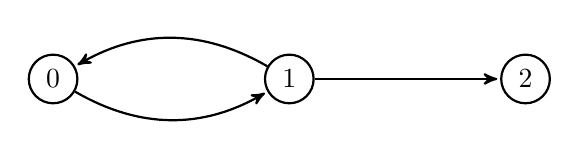
\begin{tikzpicture}[->,>=stealth',shorten >=1pt,auto,node distance=3cm,thick,main node/.style={circle,draw}]
    \node[main node] (0) {0};
    \node[main node] (1) [right of=0] {1};
    \node[main node] (2) [right of=1] {2};

    \path[every node/.style={font=\sffamily\small}]
    (0) edge [bend right] (1)
    (1) edge (2)
    (1) edge [bend right] (0);
  \end{tikzpicture}

  The first call is \texttt{allPaths(graph, 0, 2)}, which leads to \texttt{allPaths(graph, 1, 2)}, which leads back to \texttt{allPaths(graph, 0, 2)}.
\item
  \begin{lstlisting}
def allPaths(graph, source, sink):
    # `u' takes place of `source'; `graph' and `sink' are fixed;
    # `prev' maintains history
    def f(prev, u):
        result = []
        if u == sink:
            result = [u]
        else:
            # Add current node to list of visited nodes
            prev_ = [u] + prev
            # Don't consider vertices already visited
            for v in graph.verticesAdjacentTo(source) - prev:
                for path in f(prev_, v):
                    result.append([u] + path)
        return result

    return f([], source)
  \end{lstlisting}
\item
  The algorithm terminates because, in each recursive call to \texttt{f}, \texttt{prev} gains an element. \texttt{prev} is a subset of the set of vertices in \texttt{graph}, so the complement of \texttt{prev} in \texttt{graph} decreases in size with each recursive call.

  All paths output are correct paths because they all contain a sequence of connected vertices from \texttt{source} to \texttt{sink}. This can be proven by induction on the length of the path.

  All relevant paths are included in the output because all possible paths that don't revisit a node are included. In the maximum flow problem, loops have no value, so need not be included.
\end{enumerate}

\section{Jarvis' march}
\begin{enumerate}
\item Start from the rightmost point and add this to the convex hull. Measure the anticlockwise angle between vertical and each other point, with the angle being at the starting point. Move along to the point with smallest angle. Repeat from this new point, replacing the vertical with the line passing through the previous point and the current point. When the original (rightmost) point is reached again, the algorithm terminates.
\item
  \begin{enumerate}
  \item We define \(\begin{pmatrix}a\\b\end{pmatrix}\times\begin{pmatrix}c\\d\end{pmatrix}=a\cdot d-b\cdot c\). It holds that, for any 2-vectors \(\mathbf p\) and \(\mathbf q\), \(\mathrm{sign}\,(\theta\,\mathbf q\,\mathbf p)=\mathrm{sign}\,(\mathbf p\times\mathbf q)\), where \(\theta\,\mathbf q\,\mathbf p\) is the smallest (in absolute value) angle between \(\mathbf q\) and \(\mathbf p\), measuring anticlockwise as positive. This gives a way to decide whether one point lies anticlockwise or clockwise of another with respect to the origin using only elementary operations.
  \item The vectors can be sorted using a variant of Quicksort. Instead of pivoting on an item, we pivot by working out whether each vector lies anticlockwise or clockwise of a vector bisecting the sector currently under consideration. We start by comparing against \(-\mathbf i\), with anticlockwise vectors being greater than all clockwise vectors. Then, the two halves are sorted separately.
  \end{enumerate}
\end{enumerate}

\section{Flow network}
\begin{enumerate}
\item
  \begin{enumerate}
  \item A flow network is a directed graph on which edges have associated values. For each edge, this value represents the capacity of this edge, i.e, how much flow can go through it.
  \item
    A flow is a function \(f\) with the following properties:
    \begin{align}
      &f\,(u,v)=-f\,(v,u) \\
      &f\,(u,v)\leq c\,(u,v) \quad \textrm{where }c\textrm{ is the capacity between the two vertices}\\
      &\forall u\in V.\sum_{v\in V}f(u,v)=0
    \end{align}
    It is used to represent a valid amount flowing through the graph, and how that is achieved.
  \item The value of the flow, \(|f|\), is the amount flowing through the graph according to flow \(f\). This is equal to both \(\sum_{v\in V}f\,(s,v)\) and \(\sum_{u\in V}f\,(u,t)\), where \(s\) is the source vertex and \(t\) is the sink vertex.
    \setcounter{enumii}{5}
  \item An augmenting path is a sequence of consecutive edges from the residual network along which a positive flow can be found.
  \end{enumerate}
\item
  \begin{lstlisting}
def fordFulkerson(getAugmentingPath, flow, graph, source, sink):
    case getAugmentingPath(flow, graph, source, sink) of
        Nothing:
            return flow
        Just (value, edges):
            fordFulkerson(getAugmentingPath,
                          lambda e: (value if e in edges else 0) + flow(e),
                          graph, source, sink)
  \end{lstlisting}
  The worst case performance of the algorithm depends on the difference between the smallest augmenting path and residual capacity throughout execution. In the worst case, the smallest augmenting path (in terms of capacity) is chosen every time.

  The algorithm definitely terminates if all edge weights are rational. In this case, the problem can be transformed to be about solving a network with integer weights by multiplying the weight of each edge by a common multiple of the denominators. The case with all integer weights terminates because each pass of the algorithm decreases the residual flow by at least 1. When the residual flow is 0, the algorithm is finished.
\item We can't conclude that \(f_3\) is a flow because it could be the case that \(f_1=f_2\) and \(f_1\) is a maximal flow on a non-trivial network. Then, there exist edges (those on the minimum cut, for instance) for which \(f_1\,(x,y)=c\,(x,y)\). If any of these have positive flow, \(f_3\,(x,y)>c\,(x,y)\), contradicting the property (ii) of flow.
\item A maximum matching in a bipartite graph is a set of pairs of items, one from each half of the graph, of the greatest cardinality a set like this could achieve. From a bipartite graph, a flow network is formed by making all edges directed in the same direction, giving them each capacity 1, and adding a source and sink at either end of the graph, with edges of capacity 1 connecting these to each vertex in their respective half. A maximum flow of this network corresponds to a maximum matching by taking any saturated edges to be part of the matching.
\item An augmenting path with a large number of edges is created when all nodes but one from one half are paired, but there is still an augmenting path that happens to overwrite every previously established flow. This augmenting path has two edges for each node in the smaller of \(L\) and \(R\), plus an edge connecting to the source or sink. This gives an upper bound of \(\mathrm{min}\,(|L|,|R|)+1\).
\end{enumerate}

\section{Convex hull}
The situation is presumably in 3-dimensional space, in which there is no variant of Graham's scan that works. If it were in 2-dimensional space, Graham's scan probably would be used, since 1000 is much greater than \(\lg 1000000\) (which is about 20).

\section{Determinacy race}
?

\section{Sorting}
Define the less-than-or-equal operator used by the sorting algorithm to be the function \(\lambda p,q.p\times q\leq 0\). This compares vectors for angles using only multiplication, subtraction and number comparison (for whatever type of number has been chosen). To use this, compare all vectors to a vector with median angle (\(\mathbf i\) if angles are interpreted as running from \(-\pi\) to \(\pi\), or \(-\mathbf i\) if angles run from \(0\) to \(2\cdot\pi\)), then sort each half of the vectors separately.

\end{document}